\documentclass[12pt]{article}

\usepackage[portuguese]{babel}

\usepackage{graphicx}
\usepackage[section]{placeins}
\usepackage{float}
\usepackage{url}

\graphicspath{ {figures} }

\author{João Vitor Maia Neves Cordeiro}
\title{Aplicações de machine learning em IoT: uma visão sobre o estado da arte}
\date{\today}

\begin{document}

\maketitle

\begin{abstract}

O presente trabalho visa fomentar um debate sobre o estado da arte das aplicações de machine learning (ML) em tecnologias Internet of Things (IoT), a fim de dar ao leitor o material necessário para compreender a importância da multidisciplinaridade entre as mais diversas áreas da computação; O artigo está dividido da seguinte forma: uma breve introdução sobre os temas ML e IoT; uma série de exemplos práticos da interligação entre as duas áreas estudadas; e por fim uma discussão sobre o que há de mais avançado sendo desenvolvido em universidade e indústrias pelo mundo; Como metodologia para a coleta de dados foi realizada uma pesquisa bibliográfica buscando materiais publicados nos últimos 3 anos em periódicos e congressos nacionais e internacionais.

\end{abstract}

\section{Introdução}

\subsection{Motivação}

O crescente interesse nos estudos da área de machine learning vem acompanhado de uma certa confusão quanto as reais aplicação dessa tecnologia, sendo disseminada principalmente por publicações equivocadas da grande mídia \cite{maram}. Desta forma, é de extrema importância que a comunidade científica formule publicações que tenham como objetivo colaborar com a formação de uma melhor fonte de conhecimento para o público geral.

Da mesma forma, é notável que a expansão do mercado de IoT seja suportada pelo avanço das tecnologias em redes de computadores e mais recentemente pelo aprendizado de máquina.

\subsection{Justificativa}

Como será visto melhor em seguida, os dois principais conceitos trabalhados nesse artigo estão em grande foco no cenário mundial, com novas pesquisas sendo realizadas todos os dias tanto no âmbito acadêmico quanto institucional \cite{nguyen}.

Dessa forma, é essencial que sejam realizadas revisões bibliográficas sistemáticas com frequência, para verificar qual o estado atual dessas pesquisas. Somente a partir de um processo de revisão desses é possível compreender o estado da arte e definir prioridades de pesquisa futuras.

\subsection{Objetivos Gerais}

Esse artigo se propõe a introduzir alguns conceitos básicos para o melhor entendimento de seu conteúdo, discutir sobre as principais aplicações de técnicas de aprendizado de máquina em IoT bem como apontar avanços notáveis nessa área.

\subsection{Objetivos Específicos}

\begin{itemize}
    \item Introduzir ao leitor os assuntos machine learning e IoT.
    \item Listar de forma não extensiva as aplicações possíveis de técnicas de machine learning em dispositivos IoT
    \item Comentar sobre o estado da arte das já citadas aplicações, com situações reais. 
\end{itemize}

\subsection{Organização do artigo}

Este artigo está organizado da seguinte forma:

Na seção 2, conceitos básicos, temos uma breve introdução aos conceitos que serão necessários para o entendimento do trabalho, a definição e explicação de IoT e Machine Learning; Na seção 3, trabalhos correlatos estão outras obras relacionadas da área, a fim de explicar a importância das aplicações de machine learning em dispositivos IoT; Na seção 4, aspectos relevantes são permeados os assuntos importantes para a contextualização do texto. Além destes, a seção também trabalha pontos específicos que devem ser levados em consideração quando tratamos de aplicações de machine learning em dispositivos IoT; Na seção 5, problemas existentes, aqui entramos nas dificuldades e desafios associados à esta área de pesquisa; Na seção 6, soluções possíveis, busca-se apresentar soluções para os desafios propostos na quinta seção; Na seção 7, entramos a fundo no desenvolvimento da solução proposta por Sacco \emph{et al.} \cite{sacco}. Na seção 8 são apresentadas as conclusões retiradas a partir da análise da bibliografia e trabalhos futuros a serem realizados. Por fim, em referências bibliográficas estão listados todos os trabalhos utilizados como base para a confecção deste artigo, dando o devido crédito aos autores originais.

\section{Conceitos básicos}

\subsection{Machine Learning}

O termo machine learning foi cunhado por Samuel Lee Arthur, ainda na década de 50, quando Arthur trabalhava como pesquisador para a IBM desenvolvendo um programa capaz de aprender a jogar xadrez. O algoritmo em questão utilizava dados de outras partidas para prever a probabilidade de vitória a cada ação, tomando o caminho com a maior probabilidade de vitória. O termo se refere a capacidade dos algoritmos de ML de evoluirem conforme a execução, baseando-se em dados para aprender a melhor forma de realizar uma função. 

De forma mais prática, machine learning é área da ciência da computação que estuda algoritmos que podem aprimorar seu funcionamento por base de experiências prévias, sejam essas fornecidas por um banco de dados ou pelos dados que o algoritmo gera durante sua execução. É extensivamente utilizada em situações onde algoritmos convencionais não podem resolver o problema de forma satisfatória ou em tempo hábil.

\subsection{Internet of Things}

A primeira definição do termo \emph{internet of things (IoT)} veio do trabalho de Ashton \emph{et al.} e pode ser traduzido para "uma rede aberta e abrangente de objetos inteligentes que têm a capacidade de se autoorganizar, compartilhar informações, dados e recursos, reagir e agir diante de situações e mudanças no ambiente". Desde então, os "objetos inteligentes" foram renomeados para "coisas" (\emph{things}) e são descritos como dispositivos de hardware e software capaz de se conectar a uma rede com capacidade para performar uma funcionalidade específica. 

Hoje, mais de 20 anos após a primeira definição, os dispositivos IoT invadiram as casas e indústrias do mundo, adquirindo um papel essencial na sociedade moderna e que segundo recente análise \cite{analisis} está em crescente tanto em lucro quanto em produtividade. Essas tecnologias podem se espalhar por diversas áreas, sendo as mais notáveis: automação residencial, agricultura inteligente e automação industrial.

\section{Trabalhos correlatos}

A tabela a seguir contendo uma revisão bibliográfica sistêmica realizada em buscas no Scholar Google nos mostra que há uma quantidade massiva de trabalhos realizados na área de IoT e machine learning, o que também é observado quando utilizamos as duas keywords simultâneamente.

Os resultados apontam que existe um interesse global nos assuntos, com a maioria dos trabalhos sendo escritos em inglês mas espalhados em países pelo mundo todo.

\begin{center}
    \begin{tabular}{ | c | c | }
    \hline
    Keywords & Resultados \\ 
    \hline
    IoT & 1,120,000 \\  
    \hline
    Machine Learning & 4,670,000 \\
    \hline
    IoT Machine Learning & 176,000 \\
    \hline
    Machine learning applications on IoT & 161,000 \\
    \hline
    Machine learning on sensors & 1,380,000 \\
    \hline
    \end{tabular}
\end{center}

Durante o desenvolvimento desse artigo, buscamos utilizar a bibliografia pesquisada como arcabouço de conhecimento necessário para construir uma revisão sistemática e precisa do estado atual da conjuntura entre as duas grandes áreas observadas. Após identificar como um dos principais problemas a falta de uma arquitetura padrão optamos por realizar um aprofundamento nessa problemática, utilizando principalmente o artigo de Sacco et al. \cite{sacco} como base para a comparação entre as arquiteturas existentes no mercado e as que estão sendo propostas atualmente por pesquisadores da área.

\subsection{A Survey of Machine and Deep Learning Methods for Internet of Things (IoT) Security \cite{ali}}

O artigo de Mohammed Ali Al-Garadi \emph{et al}. tem como premissa a
quantidade crescente de dispositivos conectados que operam com
pouca intervenção humana para questionar a importância de se preocupar em dobro com segurança
em um contexto de IoT.

Os dispositivos IoT contam com necessidades específicas da área e muitas
vezes únicas quanto ao escopo de desenvolvimento e aplicação, por consequência disso podem acabar
deixando a desejar quando o assunto é segurança, sendo protegidas por meios comuns e menos modernos de criptografia e controle de acesso. 

Considerando isto, as técnicas de machine learning que obtiveram grandes avanços no passado recente, se
mostram ferramentas capazes de suprir as necessidades de segurança da IoT. O autor mostra, de forma direta e acessível, informações sobre as
tecnologias em machine learning aplicadas a segurança de dispositivos de IoT, criando uma base sólida de conhecimento para
auxiliar no direcionamento de futuras pesquisas do assunto.

\subsection{Crop Management with the IoT: An Interdisciplinary Survey \cite{vitali}}

O trabalho publicado por Vitali \emph{et al.} começa com uma conceituação histórica sobre a lenta evolução tecnológica da agricultura até a revolução verde, 
que acelerou vertiginosamente a inovação na área. Após isso, os autores citam a introdução dos dispositivos IoT na agricultura como uma segunda revolução verde,
junto com outras novas tecnologias que aos poucos são incorporadas nas lavouras, como \emph{machine learning} e \emph{edge computing}.

São citadas como principais causas dessa proliferação de tecnologias no campo o barateamento de constante de \emph{chips} capazes de executar as aplicações de ML, o desenvolvimento de novos sensores capazes de desempenhar suas funcionalidades com menos gasto energético e o avanço de técnicas como o \emph{deep learning}.

Os pesquisadores da universidade bolognesa ainda concluem apontando que a ampliação do uso dessas tecnologias em fazendas inteligentes é capaz de otimizar os lucros de proprietários de terras, assim como de diminuir impactos ambientais causados pelos plantios e aumentar a produção global de alimentos e insumos. Por fim, também fazem uma projeção de que em poucos anos essas tecnologias estarão nas mãos até de pequenos fazendeiros individuais continuando a melhorar a vida no campo.

\subsection{Realizing an Effective COVID-19 Diagnosis System Based on Machine Learning and IOT in Smart Hospital Environment \cite{hameed}}

Uma das áreas ainda não citada aqui mas que possui grandes incentivos para pesquisas em IoT são os Smart Hospitals, ambientes de amparo a saúde controlados por dispositivos interconectados que podem performar diversas funções, desde a captação de sintomas até a administração de medicações. Durante o ano de 2020, essas pesquisas tenderam-se a focar na pandemia do vírus SARS-COV-2, como é o caso do artigo citado.

No trabalho publicado por Abdulkareem \emph{et al.} nós temos uma pesquisa de cunho mais experimental, lidando diretamente com amostras do vírus. Segundo o texto, foram coletados dados de pacientes ao redor do mundo com a ajuda de sensores em dispositivos inteligentes. Após isso, foram treinados modelos de 3 tipos: Naive Bayes (NB), Random Forest (RF), e Support Vector Machine (SVM). Dos 3 citados, o que se saiu melhor nos testes foi o modelo SVM, com uma precisão de até 95\% em diagnósticos, sendo o sugerido pelos pesquisadores para uma possível aplicação em campo.

O artigo conclui que o modelo de ação proposto, que utiliza o Machine Learning como suporte para decisões clínicas ainda é superior aos modelos completamente automatizados, já que o fator humano continua sendo de grande importância para mitigar possíveis erros da máquina.

\subsection{An architecture for adaptive task planning in support of IoT-based machine learning applications for disaster scenarios \cite{sacco}}

Todos os anos, milhares de desastres naturais e acidentes causados por humanos acontecem pelo mundo, pondo em risco a vida não só das pessoas afetadas mas também dos profissionais responsáveis por socorrer e resgatar as vítimas dessas situações. O uso de drones para cenários como esses se tornou popular recentemente, devido ao barateamento da tecnologia utilizada para o funcionamento básico dessas máquinas. O artigo publicado por Sacco \emph{et al.} descreve as a arquitetura de uma possível aplicação de machine learning no aprimoramento desses dispositivos.

Ao alimentar algoritmos de aprendizado de máquina com dados em vídeo captados por drones em desastres é possível treinar um modelo capaz de interpretar em tempo real a situação de um novo desastre e escolher a melhor ação a ser tomada nesse caso. Em específico, a arquitetura proposta pelo trabalho lida com um cenário de múltiplos agentes semi autônomos que são programados para realizar tarefas gerais como apagar chamas, remover escombros e carregar vítimas. Após treinado, o modelo é conectado ao drone e passa a monitorar as atividades que ocorrem no ambiente ao redor dele, pronto para identificar e responder a situações de risco.

A conclusão dos pesquisadores é de que apesar de promissor, o modelo ainda conta com algumas barreiras, como a baixa precisão de sensores em situações tão extremas. É possível que com o avanço na tecnologia dos sensores, aplicações como essa possam se tornar 100\% autônomas, salvando a vida de milhares de pessoas em desastres, sem arriscar a vida de socorristas.

\section{Aspectos Relevantes}

Durante a leitura dos artigos de base foi constatada uma interdisciplinaridade intensa, tanto em problemas quanto em soluções propostas a estes. É notável o esforço de pesquisadores da área da computação para compreender assuntos que tocam outras áreas do conhecimento e assim propor abordagens inteligentes para os dilemas que surgem.

Por se tratar de uma área em ascenção, o espaço disponível para novas ideias e novas tentativas se mostra enorme, considerando que para cada uma das áreas aplicadas é possível que um algoritmo X ou Y se dê melhor para a solução proposta, com novos algoritmos sendo criados todos os dias e evoluções sendo feitas nos algoritmos existentes \cite{hameed}.

Outra coisa que chamou atenção foi a maneira como a evolução constante e barateamento de sensores impacta nos futuros trabalhos a serem desenvolvidos na área, se hoje um equipamento se mostra inviável pelo custo de produção ou pela falta de precisão no sensor é possível que em anos ou mesmo meses, com essa barreira tecnológica sendo quebrada, algoritmos e aplicações de machine learning que se mostravam ineficientes acabem se tornando o estado da arte \cite{sacco} \cite{ali}.

É interessante também comentar da alta gama de aplicações que podem utilizar os conceitos tratados nesse trabalho, frequentemente é citado por autores que seus trabalhos precisam generalizar diversos conceitos a fim de acomodar aplicações de áreas diferentes. Isso impacta no desenvolvimento de padrões e soluções gerais, pois quanto mais variáveis possíveis de serem aplicadas ao sistema, maior a complexidade exigida de um modelo e mais difícil de alcançar resultados satisfatórios.

Sacco \emph{et al.} demonstram isso em seu trabalho de forma detalhada, veremos os detalhes mais a frente, mas já se pode introduzir que ao idealizar uma arquitetura genérica para a construção de sistemas IoT com apoio de aplicações de machine learning as variáveis aparecem aos montes \cite{sacco}. O sistema precisa de respostas em tempo real? O sistema precisa estar conectado à rede mundial de computadores ou pode possuir apenas uma rede local? Quais as especificações energéticas a serem atingidas? Qual a quantidade de processamento disponível? Usaremos \emph{cloud computing} ou \emph{edge computing}?

Apenas após responder a essas e outras perguntas uma aplicação dessa gama pode começar a ser projetada, e mesmo após escolher uma arquitetura base como a APRON ou HAP é provável que alterações devam ser realizadas nessas arquiteturas para comportar corretamente o escopo da sua aplicação. Essas alterações podem ser feitas por meio de uma API fornecida pela própria arquitetura ou por modificação direta no funcionamento da arquitetura, adicionando, removendo e modificando componentes para satisfazer as necessidades do sistema a ser criado.

Ao fim, outro aspecto importante a se citar é que pelos assuntos a serem tratados nesse artigo terem um tempo de vida relativamente curto, ainda estamos possívelmente no começo de uma revolução completa no modo de vida dos seres humanos, e apesar de aspectos éticos e de segurança ainda serem preocupações importantes, as tecnologias estudadas vem se mostrando com usos impressionantes para o auxílio no crescimento do nosso padrão de vida.

\section{Problemas Existentes}

Foi possível identificar durante a leitura dos trabalhos correlatos que existem problemas de certa forma estão interconectados, na maior parte limitações de hardware. Nessa seção, esses problemas serão esmiuçados para futura análise e proposição de soluções. O primeiro problema a ser citado foi termo comum entre a maior parte das publicações analisadas, a relação entre custo dos sensores e a precisão das medições.

Algoritmos de machine learning precisam de dados extremamente precisos, tanto durante o treinamento do modelo quanto durante sua execução, tendo isso em vista é necessário que os sensores que irão captar os dados utilizados pelos modelos tenham uma precisão satisfatória. Entretanto, quanto mais preciso o sensor, mais pesado para o bolso de quem irá custear o projeto e a produção. É normal que no impulso para economizar nos sensores os fabricantes maiores de dispositivos IoT acabem negligenciando essa precisão, o que não pode de maneira nenhuma ocorrer em cenários de serviços críticos com aplicações de machine learning \cite{sacco}.

Outra dificuldade relacionada ao hardware dos sistemas que é apontada por diversos autores é falta de poder computacional que a maior parte dos dispositivos IoT, o que faz com que os modelos tenham que ser rodados em servidores remotos com o auxílio de \emph{cloud computing}, impactando no tempo de resposta (pois mesmo que a latência seja baixa, o tempo de upload e download dos dados já pode alterar significativamente a performance do algoritmo e do sistema como um todo). Por outro lado, dispositivos que possuem maior poder computacional, além de terem acréscimo no preço também precisam de mais energia para funcionar, aumentando o tamanho e custo dos dispositivos significativamente.

Outro problema conhecido e explorado por diversos autores é a preocupação quanto a segurança dos dispositivos, já que os mesmos possuem capacidades limitadas de criptografia e estão sujeitos a ataques maliciosos por utilizarem autenticações mais simples. O problema explorado por Ali \emph{et at} \cite{ali} não possui ainda uma solução definitiva, tendo em vista de que ele surge da própria natureza e definição de um dispositivo IoT. Sendo assim, somente soluções parciais ou restritas a poucos casos de uso foram implementadas e pesquisadas até o momento.

Algoritmos de machine learning precisam de dados extremamente precisos, tanto durante o treinamento do modelo quanto durante sua execução, tendo isso em vista é necessário que os sensores que irão captar os dados utilizados pelos modelos tenham uma precisão satisfatória. Entretanto, quanto mais preciso o sensor, mais pesado para o bolso de quem irá custear o projeto e a produção. É normal que no impulso para economizar nos sensores os fabricantes maiores de dispositivos IoT acabem negligenciando essa precisão, o que não pode de maneira nenhuma ocorrer em cenários de serviços críticos com aplicações de machine learning \cite{sacco}.

Por último, vale ressaltar a problemática a ser melhor explorada em seguida por esse presente artigo, é evidenciada por diversos autores \cite{sacco} \cite{ali} a falta de pelo menos uma arquitetura padronizada ou no mínimo bem aceita tanto pela comunidade científica quanto industrial. Por ser uma área em crescimento mas ainda nos seus primeiros estágios, é completamente natural que não se tenham criados padrões sólidos, mas analisando o material lido fica claro que existem boas candidatas a arquiteturas padrão sendo documentadas pela comunidade científica mas que ainda não atingiram o mundo corporativo.

Até o final desse artigo teremos passado por pelo menos duas dessas arquiteturas, com experimentos controlados mostrando sua eficiência em campo para um subset de aplicações que utilizam o apoio de machine learning. As duas arquiteturas utilizam os mesmos conceitos que exemplificamos até agora, propondo a transição de \emph{cloud computing} para \emph{edge computing}, a aplicação de novos algoritmos após essa transição para refinar e otimizar os resultados gerados por esses sistemas \cite{sacco}.

\section{Soluções Possíveis}

Por tratar-se de uma área ampla, com diversos problemas que não foram citados na seção anterior por terem menor relevância ou possuírem pouco material base de pesquisa, aqui iremos apenas propor algumas soluções possíveis para uma listagem não extensiva dos principais problemas do campo de estudo. Começaremos abordando o problema do poder de processamento citado acima, onde os dispositivos IoT por serem costumeiramente mais simples podem não conseguem executar as aplicações de machine learning.

Primeiramente vamos dividir os serviços entre dois tipos, aqueles que precisam de resultados em tempo real (usaremos aqui o critério de resultados em tempo menor do que 1s) e aqueles que podem receber os resultados em um outro momento ou que não precisam de resultado algum. Nessa solução iremos tratar apenas do primeiro grupo, tendo em vista que para o segundo grupo um simples processamento na \emph{cloud} é o suficiente para uma solução aceitável. A abordagem proposta por alguns autores e reforçada no presente artigo é a utilização de conceitos e práticas de \emph{edge computing} \cite{vitali}.

Edge computing é um paradigma de computação distribuída que traz o poder computacional e o armazenamento para perto de onde a solução é necessária, melhorando o tempo de resposta média das aplicações (por reduzir a latência) e diminuindo o uso de banda. Conceitos de \emph{edge computing} já são utilizados em algumas redes de dispositivos IoT para diminuir o custo de processamento e o gasto energético, entretanto durante a pesquisa realizada para esse artigo foram encontradas poucas menções ao seu uso para suportar aplicações de machine learning \cite{vitali}.

Prevê-se que a utilização de um servidor local na rede dos dispositivos IoT possa reduzir drásticamente o custo e tempo de cada requisição feita pelos sensores, tendo em vista que além da latência mais baixa, podemos utilizar protocolos diferentes já que não iremos utilizar propriamente a \emph{world wide web} e o HTTP, mas sim uma LAN que possui taxa de transferência superior. Além disso, ao utilizar essa abordagem o suporte dado ao usuário é melhorado, tendo em vista que normalmente ao utilizar \emph{cloud computing} são usados parques de computadores terceirizados, enquanto ao utilizar \emph{edge computing} as máquinas já estão próximas do local de uso.

Seguindo para o problema da falta de uma arquitetura padrão para o desenvolvimento dos sistemas IoT, entraremos em mais detalhes na seção "Projeto e Desenvolvimento de uma Proposta" do artigo, mas já se pode adiantar que uma arquitetura para a toda a gama de aplicações que podem utilizar suporte de machine learning em sistemas IoT deve ser pensada de forma a ter componentes customizáveis e interfaces de programação claras e genéricas. Dessa forma, a arquitetura deve ser tratada como uma base a ser modificada e complementada conforme as necessidades da aplicação hospedeira \cite{sacco}.

Podemos já vislumbrar o modo pelo qual a execução de novos sistemas IoT promove a alavancagem das novas proposições. Todas estas questões, devidamente ponderadas, levantam dúvidas sobre se a percepção das dificuldades acelera o levantamento das variáveis envolvidas. Percebemos, cada vez mais, que a estrutura atual das arquiteturas não pode mais comportar as mais diversas aplicações com diversas motivações. O cuidado em identificar pontos críticos na determinação clara de objetivos e metas facilita a criação das direções preferenciais no sentido do progresso em busca de uma arquitetura mais completa.

\section{Projeto e Desenvolvimento de uma Proposta}

\cite{sacco} Apresenta uma alternativa de arquitetura para sistemas IoT que exijam respostas em tempo real, focado em situações de desastres (naturais ou causados por ação humana), mas que também pode ser extendido e aplicado para uma gama maior de serviços, sendo citados pelos autores as áreas de transporte inteligente e cidades inteligentes. Sacco \emph{et. al} propõem o uso da arquitetura APRON (Architecture for the Programmability of RObotic Networks) para generalizar e trabalhar o problema com enfoque no uso de Unmanned Aerial Vehicles (UAVs, ou simplesmente drones), desenvolvida pelos autores para habilitar empresas e projetistas à produzir novas soluções focadas em áreas específicas.

A arquitetura proposta conta com diversas ferramentas \emph{out of the box} para auxílio no desenvolvimento das soluções, além de obviamente permitir que novas ferramentas sejam implementadas e adicionadas ao sistema. Como exemplo de ferramentas citadas pelos pesquisadores temos monitoramento da rede, reparação e controle de agentes, busca de agentes vizinhos/próximos, filas de tarefas e estimativa de falha de tarefas.

Os autores apresentam uma arquitetura rica e completa em ferramentas, que trabalha numa camada intermediária entre o sistema operacional do \emph{cloudlet} e as aplicações (controladores dos dispositivos IoT e aplicações de machine learning). Dentro da própria APRON temos diversos componentes que podem ser vistos na figura abaixo, com destaque para o Mission Planning Controller que é detalhado em minúcias no artigo publicado.

\begin{figure}[H]
    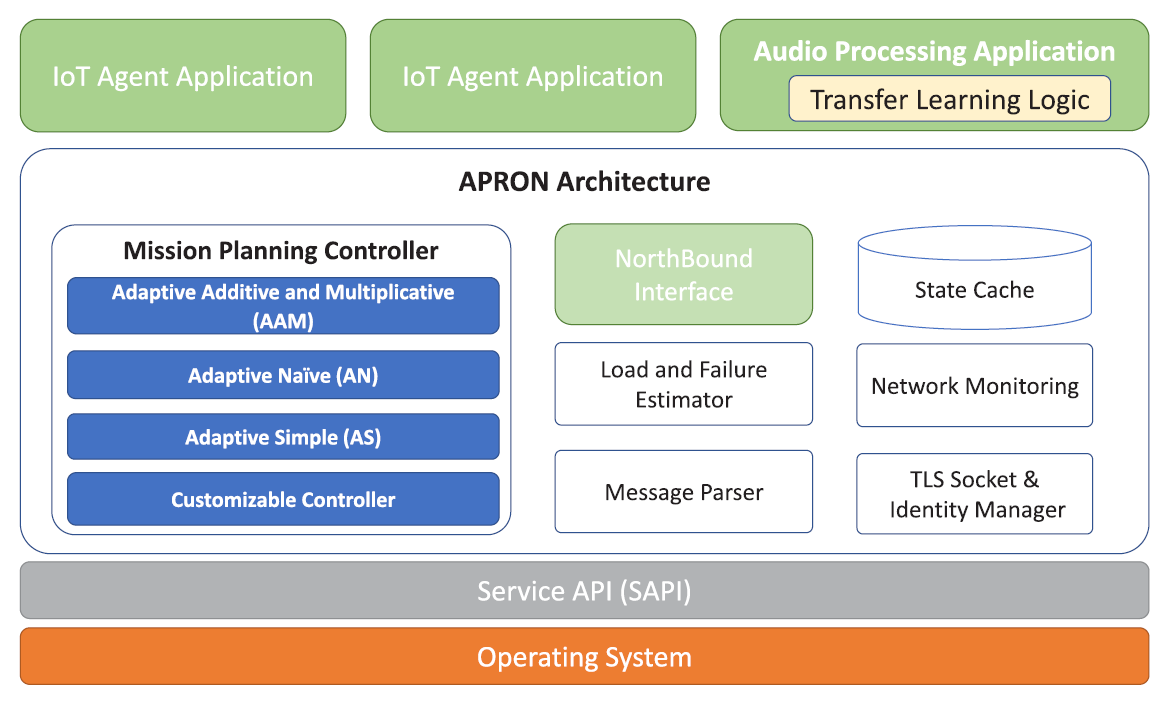
\includegraphics[width=\linewidth]{apron.png}
    \caption{APRON: uma camada de gerenciamento entre a aplicação IoT e o sistema operacional, feita para estabelecer e monitorar conexão entre agentes, estimar taxas de falhas dos agentes, adaptar-se a tarefas e planejar a lógica de controle de missão \cite{sacco}.}
\end{figure}

\subsection{Missiong Planing Controller}

É amplamente disseminado entre publicações da área que provavelmente não encontraremos uma solução universal para problemas que envolvem modelos atuando em cenários de mundo real, portanto o máximo que os autores costumam buscar é uma abordagem ampla o suficiente para poder ser aplicada em alguns cenários com uma taxa aceitável de erros.

Os autores explicam a forma como o modelo de planejamento trabalha utilizando uma \emph{Jackson Network} que demonstra a fila de tarefas sendo distríbuidas, onde podem existir N nodos (ou agentes) na rede capazes de performar uma ou mais classes de tarefas. Cada nodo recebe uma quantidade balanceada do total de tarefas, respeitando as classes. Caso o sistema detecte uma falha em qualquer nodo, as tarefas são redistribuídas, respeitando novamente as classes e ordens.

\subsection{Network Monitoring}

Inspirado em outros modelos clássicos, o componente de monitoramento de rede da APRON utiliza um protocolo próprio de descobrimento de rede descolado do TCP/IP, portanto não possui os problemas decorrentes da faixa limitada de endereços IPV4. Os agentes possuem um endereço único e são monitorados continuamente com algo parecido com um \emph{ping} para verificar se ainda estão conectados.

\subsection{Service API}

Esse componente é o que extende a customização da arquitetura para diversas aplicações diversas, tendo como foco a customização de duas funções principais: a lógica do controlador de cenários e o algoritmo de planejamento de missão apresentado anteriormente. Dessa forma, é possível fazer com que a arquitetura APRON se adapte a situações diversas apenas sobrescrevendo esses comportamentos padrões para se aproximarem do cenário desejado pelo desenvolvedor de aplicação.

\subsection{Aplicação: Drone-sourced live audio analytic}

Os pesquisadores aplicaram a arquitetura descrita para uma aplicação no seguinte cenário: um \emph{swarm} de drones (nossos dispositivos IoT) vasculham uma área após um desastre natural, gravando o áudio das redondezas e enviando para o \emph{cloudlet} que roda uma aplicação de machine learning capaz de decodificar e analisar o áudio em busca de vozes humanas. Ao encontrar uma fonte de voz humana, o servidor central envia a localização aproximada da fonte para um segundo tipo de drone, esse com capacidade para realizar o resgate.

Nesse caso, temos uma latência baixa por ser tratar de uma aplicação utilizando \emph{edge computing}, e um processamento forte o suficiente para utilizarmos técnicas de redes neurais e NLP. A aplicação foi treinada utilizando sons de ambientes naturais, sons causados por desastres e por último, sons causados por seres humanos. Foram utilizadas 2000 amostras de sons, cada uma contendo 5 segundos de gravação e a rede pré treinada VGGish \cite{hershey}.

Para os testes foram utilizadas simulações contendo 10, 50 100, ou 150 drones e com distância entre pontos de interesse (pontos onde os drones deveriam visitar) variando como 1, 2, 3, 5, ou 10 metros. Além disso, 3 hipóteses foram testadas quanto ao planejamento: a primeira não rebalanceia tarefas em caso de erro, a segunda possui um threshold randômico de erros e rebalanceia as tarefas de forma aleatória, a última hipótese também possui um threshold randômico de erros mas rebalanceia as tarefas considerando os drones mais próximos daquele que falhou.

Após as simulações terem sido executadas, os pesquisadores ao analisar os dados concluíram que tanto a segunda quanto a terceira hipótese concluem a missão em um tempo mais curto, mas que a abordagem de rebalancear as tarefas para drones mais próximos daquele que falhou apesar de ser mais custosa em termos de processamento, traz melhores resultados em tempo de missão.

\begin{figure}[H]
    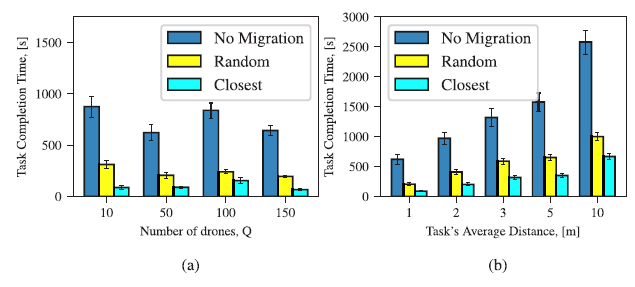
\includegraphics[width=\linewidth]{results_1.png}
    \caption{Dados resultantes da simulação.}
\end{figure}

Também foram realizadas simulações comparando a APRON com uma outra solução de mesmo escopo, a HAP, que possui uma modelagem mais complexa mas não é capaz de suportar muitos agentes simultâneos. Nas simulações a HAP apresentou uma taxa de falhas ligeiramente maior do que a APRON, mas lembrando que tratamos de aplicações críticas, qualquer taxa de falhas a mais pode resultar em perda de vidas humanas

\begin{figure}[H]
    \centering
    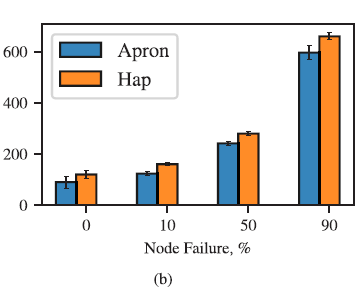
\includegraphics[width=0.5\linewidth]{apron_vs_hap.png}
    \caption{Comparação da APRON e HAP.}
\end{figure}

Os autores terminam concluindo que a proposta de arquitetura se mostrou validada no cenário para a qual foi testada, e que por sua versatilidade pode ser moldada para atuar em outras áreas sem perca de conteúdo ou eficiência. Pontuam ainda que a programabilidade e replanejamento de tarefas obtida ao se utilizar a APRON é essencial para aplicações que são implantadas em situações que envolvam ambientes com um alto grau de imprevisibilidade.

\section{Conclusões e Futuros Trabalhos}

Ao analisar uma pequena fração da ampla gama disponível de artigos e periódicos relacionados ao assunto estudado conseguimos obter um panomara inicial do estado da arte, retirando conclusões que ainda podem ser remodeladas posteriormente. Os problemas encontrados ao ler os materiais apontam para a necessidade do avanço e modernização da área de sensores, para aumentar a precisão dos dados utilizados pelos algoritmos de machine learning, e para a urgência na maior difusão de arquiteturas baseadas em conceitos de \emph{edge computing} para aplicações de alto desempenho em tempo real.

Como trabalhos futuros, destaca-se a possibilidade de modelar e validar uma arquitetura genérica para aplicações que necessitam de um tempo de resposta excepcional, pesquisando sobre arquiteturas já existentes, identificando pontos fracos e fortes delas, a fim de construir um novo padrão capaz de se adaptar a uma boa gama de aplicações com pouca ou nenhuma modificação em si mesmo.

\nocite{*}
\medskip

\bibliographystyle{ieeetr}
\bibliography{biblio}

\end{document}